\chapter{Cuestionario} \label{Ap:cuestionario}

% the code below specifies where the figures are stored
\ifpdf
    \graphicspath{{Apendice/figures/PNG/}{Apendice/figures/PDF/}{Apendice/figures/}}
\else
    \graphicspath{{Apendice/figures/EPS/}{Apendice/figures/}}
\fi



\global\mdfdefinestyle{cuestionarioST}{%
linecolor=blue,linewidth=2pt,%
leftmargin=1cm,rightmargin=1cm
}

\global\mdfdefinestyle{hipotesis0}{%
linecolor=black,linewidth=1pt,%
leftmargin=1cm,rightmargin=1cm
}
Este apéndice contiene el cuestionario utilizado para la evaluación de EvalCourse mediante un estudio de caso de ejemplo que muestra la extracción de indicadores del wiki de Moodle. Además, en un segundo apartado se analizan las respuestas recogidas. Las secciones de este apéndice son:

\begin{itemize}
	\item Cuestionario (ver sección~\ref{apc:sec:cuestionario})
	\item Resultados  (ver sección~\ref{apc:sec:resultados})
\end{itemize}

\newpage

\section{Cuestionario} \label{apc:sec:cuestionario}
	
	\subsection*{A. Nivel educativo}

\begin{mdframed}[style=cuestionarioST]
		Indique el nivel educativo en el que imparte su docencia:
			\begin{itemize}
				\item Infantil
				\item Primaria
				\item Secundaria
				\item Superior
				\item Otras
			\end{itemize}
\end{mdframed}

	\subsection*{B. Conocimientos de programación}

\begin{mdframed}[style=cuestionarioST]
			Indique los conocimientos de programación que considera que posee:
			\begin{itemize}
				\item Nulos
				\item Muy básicos
				\item Básicos
				\item Medios/avanzados
			\end{itemize}
\end{mdframed}

	
	%EvalCourse es un programa que mediante una consulta nos ofrece indicadores del trabajo de los estudiantes en el Wiki.

	\subsection*{C. Consultas de indicadores}

\begin{mdframed}[style=cuestionarioST]
	Se muestran dos consultas y las figuras obtenidas mediante EvalCourse. Los tres estudiantes que se mencionan trabajaron en una página del wiki entre las semanas 38 y 50 del curso, momento en que el trabajo debía estar terminado.
\end{mdframed}

\newpage

	\paragraph*{C.1 Consulta de indicadores 1}

\begin{mdframed}[style=cuestionarioST]
			A la vista de la figura~\ref{fig:SantaPie} obtenida con la consulta~\ref{code:apconsulta1}: ¿Sería capaz de valorar si los tres estudiantes han participado activamente en el wiki?
			\begin{itemize}
				\item Sí
				\item No
			\end{itemize}

			\rule{30mm}{1pt} \newline
\begin{lstlisting}[caption=Consulta participación de los estudiantes en el wiki,label=code:apconsulta1, captionpos=b, morekeywords={Evidence,get, students, show, milestones, participation, access, in, assignment, forum, campus, wiki, between, and, workshop, interaction, assessment, grade, from, course, backup}]
Evidence Participacion: 
	get students 
	show participation 
	in wiki.
\end{lstlisting}
\end{mdframed}

\begin{figure}[h]
 \begin{center}
    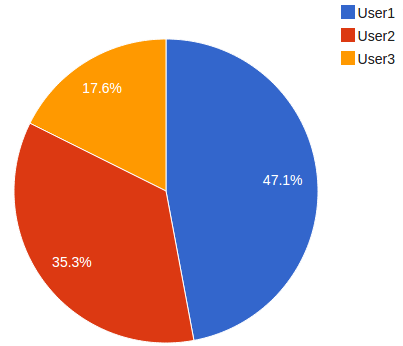
\includegraphics[scale=0.65]{santa_pie.png}
  \end{center}
  \caption{Participación de los estudiantes en la página del wiki}
  \label{fig:SantaPie}
\end{figure}

\newpage

%		\subsection*{Contribuciones aportadas por los estudiantes a lo largo del curso a la página del wiki}




%		\subsection*{Evolución del contenido aportado por los estudiantes a su página del wiki}

	\paragraph*{C.2 Consulta de indicadores 2}

\begin{mdframed}[style=cuestionarioST]

			A la vista de las figuras~\ref{fig:SantaContribuciones} y~\ref{fig:SantaEvolucion} obtenidos mediante la consulta~\ref{code:apconsulta2}: ¿Sería capaz de valorar si los estudiantes contribuyeron al wiki de forma continua?
			\begin{itemize}
				\item Sí
				\item No
			\end{itemize}

			\rule{30mm}{1pt} \newline

\begin{lstlisting}[caption=Consulta contribuciones de los estudiantes en el wiki,label=code:apconsulta2, captionpos=b, morekeywords={Evidence,get, students, show, milestones, participation, access, in, assignment, forum, campus, wiki, between, and, workshop, interaction, assessment, grade, from, course, backup}]
Evidence Contribuciones: 
	get students 
	show interaction 
	in wiki.
\end{lstlisting}
\end{mdframed}

\begin{figure}[h]
  \begin{center}
    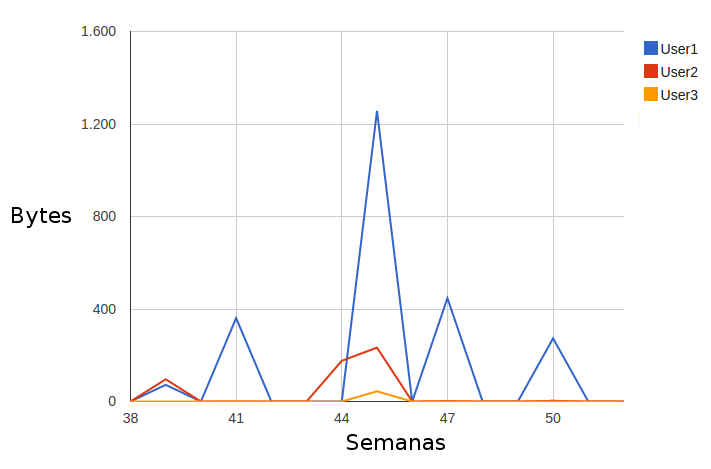
\includegraphics[scale=0.5]{santa_contribuciones.png}
  \end{center}
  \caption{Contribuciones de los estudiantes a la página del wiki}
  \label{fig:SantaContribuciones}
\end{figure}

\newpage

\begin{figure}[h]
  \begin{center}
    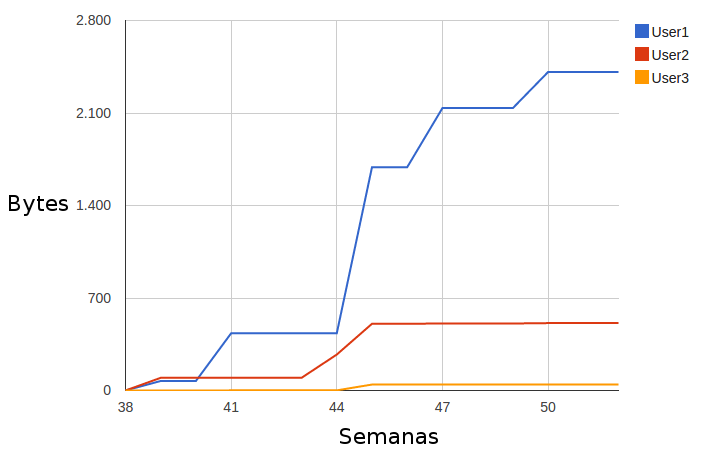
\includegraphics[scale=0.5]{santa_evolution.png}
  \end{center}
  \caption{Evolución del contenido de una página del wiki}
  \label{fig:SantaEvolucion}
\end{figure}

	\subsection*{D. Competencias evaluables}

\begin{mdframed}[style=cuestionarioST]
			Indique para evaluar qué competencias serían de utilidad los gráficos generados anteriormente.

			\rule{30mm}{1pt} \newline			

			Competencia de trabajo en equipo:
			\begin{itemize}
				\item Sí
				\item No
			\end{itemize}

			¿Por qué? \newline
			Explique por qué considera que sí o no sería posible evaluar la competencia de trabajo en equipo en el wiki a partir de los gráficos anteriores:\newline
			\rule{120mm}{1pt} \newline
			\rule{120mm}{1pt} \newline
			\bigskip

			Competencia de planificación y gestión del tiempo:
			\begin{itemize}
				\item Sí
				\item No
			\end{itemize}

			¿Por qué? \newline
			Explique por qué considera que sí o no sería posible evaluar la competencia de planificación y gestión del tiempo en el wiki a partir de los gráficos anteriores:\newline
			\rule{120mm}{1pt} \newline
			\rule{120mm}{1pt} \newline
			\bigskip

			Competencia de liderazgo
			\begin{itemize}
				\item Sí
				\item No
			\end{itemize}

			¿Por qué? \newline
			Explique por qué considera que sí o no sería posible evaluar la competencia de liderazgo en el wiki a partir de los gráficos anteriores:\newline
			\rule{120mm}{1pt} \newline
			\rule{120mm}{1pt} \newline
\end{mdframed}

\newpage

\section{Resultados} \label{apc:sec:resultados}

En esta sección se muestran y analizan en detalle los resultados del cuestionario. %Los comentarios sobre los resultados de los profesores se muestran en el capítulo X (esto se dice en la tesis de la uoc, tendré que ver qué comento yo).

\subsection{Poblaciones}

En este cuestionario participaron cuatro tipos de poblaciones. A cada una de ellas se le ha presentado el método DBA y la herramienta EvalCourse en un contexto diferente y con un nivel de detalle diferente, impuesto este por el foro en el que se presentaba. A continuación se presentan cada una de estas poblaciones y el feedback con el que respondieron el cuestionario.

\subsubsection{Curso innovación docente}
Profesorado de la Universidad de Cádiz que participó en el curso de innovación docente sobre wikis.
	\begin{itemize}
		\item{Forma de presentación:} Curso presencial.

		\item{Organización:} Dos sesiones de 4 horas cada una en la que se explicaba cómo trabajar en clase con wikis, se propusieron enfoques para favorecer el desempeño de competencias genéricas de los estudiantes y se presentaba el método DBA y la herramienta EvalCourse.  Además, se incluyeron actividades prácticas que se desarrollaron en las mismas sesiones.

		\item{Número de participantes:} 11
	\end{itemize}

\subsubsection{Taller Aulablog}
Profesorado a nivel nacional que asistió al taller sobre wikis en educación que se presentó en el encuentro de profesorado Aulablog 2015.

	\begin{itemize}
		\item{Forma de presentación:} Taller presencial.

		\item{Organización:} Una sesión de 3 horas en la que se explicó cómo trabajar en clase con wikis, se proponían enfoques para favorecer el desempeño de competencias genéricas de los estudiantes y se presentaba el método DBA y la herramienta EvalCourse.

		\item{Número de participantes:} 14
	\end{itemize}

\subsubsection{Actuación avalada}
Profesorado de la Universidad de Cádiz que participó en la actuación avalada sobre el uso de wikis.

	\begin{itemize}
		\item{Forma de presentación:} Entrevista personal.

		\item{Organización:} Se explicó a los participantes el método DBA y se les invitó a utilizar actividades en sus cursos virtuales que favoreciesen la actividad de los estudiantes en el curso para aplicar después EvalCourse. Se hizo especial hincapié en la inclusión de wikis en sus cursos virtuales. 

		\item{Número de participantes:} 7
	\end{itemize}

\subsubsection{MediaWiki}
Miembros de MediaWiki España que fueron invitados y aceptaron participar en el cuestionario.

	\begin{itemize}
		\item{Forma de presentación:} Correo electrónico.

		\item{Organización:} Mediante correo electrónico enviado a los miembros de MediaWiki España, se les explica el método DBA, la herramienta EvalCourse y se les invita a completar el cuestionario.

		\item{Número de participantes:} 19 % 1 de ellos no es mediawiki es L.Anido
	\end{itemize}

En total son 51 cuestionarios completados, repartidos tal y cómo se resume en la tabla~\ref{tab:ap:poblaciones:barras}.

\begin{table}
  \begin{center}
  \begin{tabular}{| m{5cm} | c | c |}
    \hline
    POBLACIÓN & CUESTIONARIOS & PORCENTAJE \\
    \hline
    \hline
    Curso innovación docente & 11 & 21,57\percentage \\
    \hline
    Taller Aulablog & 14 & 27,45\percentage \\
    \hline
    Actuación avalada & 7 & 13,73\percentage \\
    \hline
    MediaWiki & 19 & 37,25\percentage \\
    \hline
  \end{tabular}
\end{center}
\caption{Resumen de participantes en el cuestionario}
\label{tab:ap:poblaciones:barras}
\end{table}

\subsection{Participantes}

Como se muestra en la tabla~\ref{tab:ap:perfil:barras}, los participantes en el cuestionario cuentan con diferentes perfiles. Por un lado nos encontramos con profesores tanto universitarios (41\percentage), como no universitario (23\percentage), es decir, de infantil, primaria o secundaria. Por otro lado han participado en el cuestionario profesionales que no son profesores (35\percentage), pero que tiene un profundo conocimiento en el uso de wikis, ya que son componente de MediaWiki España. 

Además, los conocimientos de programación no deben ser un requisito de los usuarios que utilicen el método DBA y EvalCourse, por lo que se ha tratado de contar con usuarios con un nivel de programación medio o alto (49\percentage), como con conocimientos de programación nulos o básicos (51\percentage). 

\begin{table}
  \begin{center}
  \begin{tabular}{| c | m{3cm} | c | c | c | c | c |}
    \hline
     &  \multirow{3}{2cm}{\centering POBLACIÓN}  & \multirow{3}{1.7cm}{\centering Curso innovación docente}   & \multirow{3}{1.4cm}{\centering Taller Aulablog}  & \multirow{3}{1.55cm}{\centering  Actuación avalada} &  \multirow{3}{0.95cm}{\centering Media Wiki}  &  \multirow{3}{0.7cm}{\centering Total} \\
     &   &    &   &  &  &  \\
     &  &    &   &   &  &  \\
    \hline
    \hline
     \multirow{2}{2.5cm}{Conocimientos programación} & Nulos/básicos & 11 & 9 & 0 & 6 & 26 (51\percentage) \\
    \cline{2-7}
      & Medios/avanzados & 0 & 5 & 7 & 13 & 25 (49\percentage) \\
    \hline
	\hline
     & totales & 11 & 14 & 7 & 19 & 51 \\
	\hline
    \hline
     \multirow{3}{2.5cm}{Profesorado} & Universitario & 11 & 2 & 7 & 1 & 21 (41\percentage) \\
    \cline{2-7}
      & No universitario & 0 & 12 & 0 & 0 & 12 (23\percentage)\\
    \cline{2-7}
     & No profesorado & 0 & 0 & 0 & 18 & 18 (35\percentage)\\
    \hline
  \end{tabular}
\end{center}
\caption{Perfil de los participantes en el cuestionario}
\label{tab:ap:perfil:barras}
\end{table}

\subsection{Indicadores de participación y de contribución}

En este cuestionario se proponen dos consultas escritas en el lenguaje SASQL, los resultados de ejecutarlas en EvalCourse y se pregunta, en primer lugar, si se identifican los resultados de cada consulta como posibles los indicadores de la participación y de la contribución de cada estudiante al wiki.

El objetivo de esta primera pregunta de cada consulta es conocer si el participante identifica los resultados devueltos por EvalCourse como indicadores de la actividad de los estudiantes referidos a la participación y a la contribución de estos al wiki. En la tabla~\ref{tab:ap:sino:participacion:contribucion} puede verse cómo de los 51 encuestados la mayoría aceptan los resultados como indicadores de participación (82\percentage) o contribución (88\percentage). 

\begin{table}
  \begin{center}
  \begin{tabular}{| c | c | c | }
    \hline
    Respuesta & Indicador de participación & Indicador de contribución \\
    \hline
    \hline
    Sí &  42 (82\percentage) & 45 (88\percentage) \\
    \hline
    No & 9 (18\percentage) & 6 (22\percentage) \\
    \hline
  \end{tabular}
\end{center}
\caption{Respuestas dadas a la consideración como indicadores de actividad}
\label{tab:ap:sino:participacion:contribucion}
\end{table}

A partir de este punto se pasa a la evaluación de competencias genéricas, donde los participantes indicarán si consideran estos indicadores para la evaluación de competencias genéricas.

\subsection{Caso de evaluación de competencias genéricas}

Los participantes deberán responder a diferentes preguntas sobre si utilizarían los indicadores obtenidos para evaluar tres competencias genéricas de los estudiantes:

\begin{itemize}
\item Trabajo en equipo
\item Planificación y gestión del tiempo
\item Liderazgo
\end{itemize}

%Con esta pregunta se pretende deducir si el hecho de aceptar o no los indicadores está ligado exclusivamente al criterio profesor, y no  

El resumen de las respuestas dadas puede verse en la tabla~\ref{tab:ap:resumen:competencias}. En las subsecciones siguientes se describirán en detalle las respuestas para cada uno de los grupos de participantes.

\begin{table}
  \begin{center}
  \begin{tabular}{| c | c | c | c |}
    \hline
    Respuesta & Trabajo en equipo & Planificación y gestión del tiempo & Liderazgo \\
    \hline
    \hline
    Sí & 26 (51\percentage) & 40 (78,4\percentage) & 17 (33,3\percentage)  \\
    \hline
    No & 25 (49\percentage) & 11 (21,6\percentage) & 34 (66,7\percentage) \\
    \hline
  \end{tabular}
\end{center}
\caption{Resumen de la validez dada por los participantes a los indicadores para evaluar competencias genéricas}
\label{tab:ap:resumen:competencias}
\end{table}



\subsubsection{Conocimientos de programación}

¿Que los indicadores de competencias genéricas sean o no válidos para el usuario de EvalCourse es independiente de sus conocimientos de programación? Para responder a esta pregunta se analizan las respuestas dadas a cada una de las tres competencias genéricas con respecto a los conocimientos de programación, y se parte de la hipótesis nula de que ambos valores son independientes.

\paragraph*{Trabajo en equipo}

En la figura~\ref{fig:app:barras:programacion:equipo} se pueden ver las respuestas de los participantes a si utilizarían o no el indicador proporcionado para evaluar el trabajo en equipo de los usuarios del wiki en base a sus conocimientos de programación.

\begin{figure}
  \begin{center}
    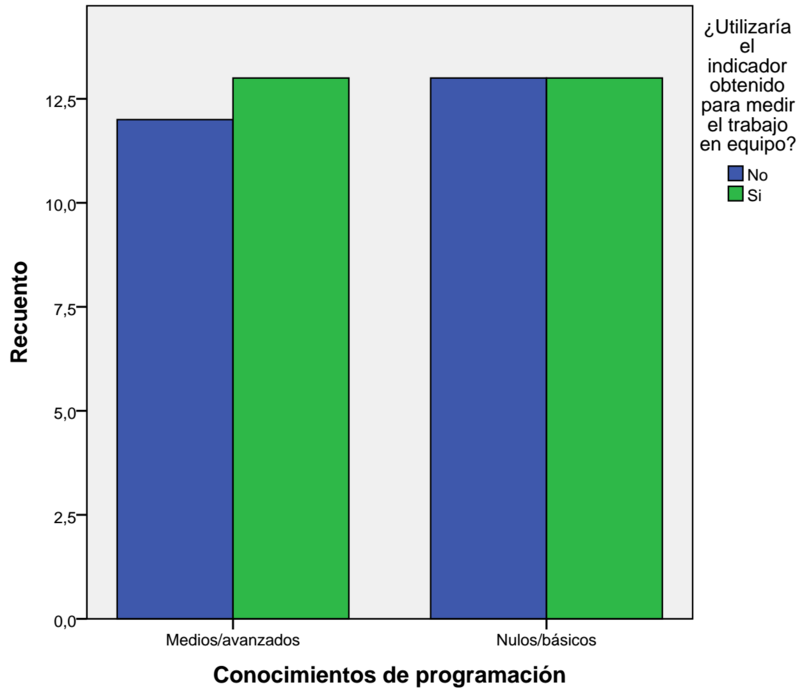
\includegraphics[scale=0.3]{barras_programacion_equipo.png}
  \end{center}
  \caption{Utilizaría el indicador para evaluar el trabajo en equipo}
  \label{fig:app:barras:programacion:equipo}
\end{figure}

Para demostrar la independencia entre los conocimientos de programación y la validez que da cada participante al indicador para evaluar dicha competencia vamos a definir la siguiente hipótesis nula:

\begin{mdframed}[style=hipotesis0]
$H_0$: \emph{Los \textbf{conocimientos de programación} son independientes de que el individuo considere que les son válidos los indicadores extraídos para medir la competencia de \textbf{trabajo en equipo}}
\end{mdframed}

Para contrastar la hipótesis nula se utilizará la prueba de chi-cuadrado. Se construye la tabla de contingencia y se calculan las frecuencias esperadas, obteniéndose el siguiente valor de chi-cuadrado ($\chi^2_0$): 

\begin{center}
	\framebox[1.2\width]{$\chi^2_0 = 0,02$}
\end{center}

Para contrastar la hipótesis se utiliza un nivel de significación del 5\percentage, siendo este valor 3,84. 

\begin{center}
	\framebox[1.2\width]{$\chi^2_{\alpha (r-1)(c-1)} = \chi^2_{0,05 (2-1)(2-1)} = 3,84$}
\end{center}

Como 0,02 es menor que 3,84 no se rechaza la hipótesis nula, y se concluye que con una significación del 5\percentage los datos son independientes.

\begin{center}
	\framebox[1.2\width]{$\chi^2_0 \leq \chi^2_{0,05 (2-1)(2-1)} \Rightarrow  0,02 \leq 3,84$}
\end{center}

\paragraph*{Planificación y gestión del tiempo}

En la figura~\ref{fig:app:barras:programacion:planificacion} se pueden ver las respuestas de los participantes a si utilizarían o no el indicador proporcionado para evaluar la planificación y gestión del tiempo de los usuarios del wiki en base a sus conocimientos de programación.

\begin{figure}
  \begin{center}
    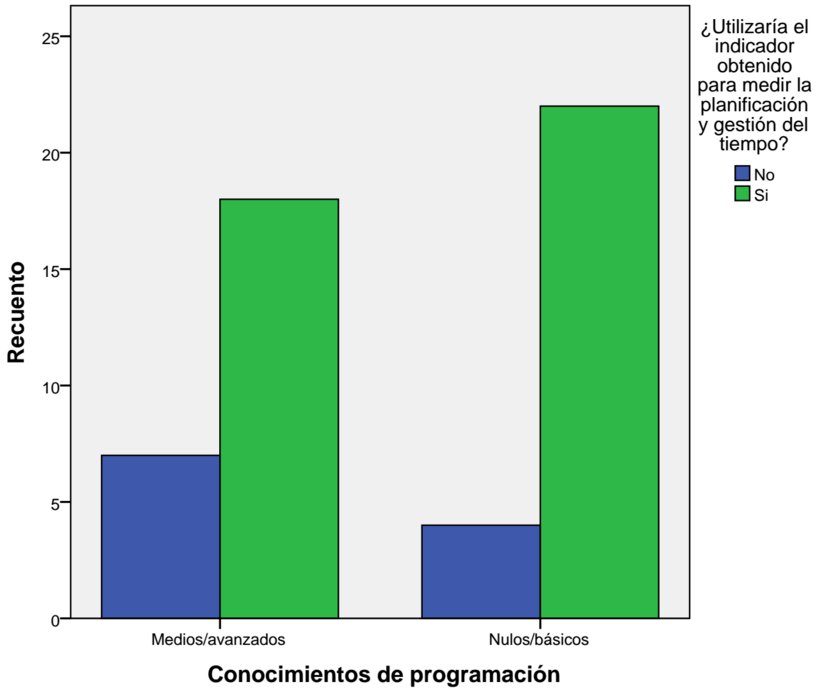
\includegraphics[scale=0.3]{barras_programacion_planificacion.png}
  \end{center}
  \caption{Utilizaría el indicador para evaluar la planificación y gestión de tiempo}
  \label{fig:app:barras:programacion:planificacion}
\end{figure}

Para demostrar la independencia entre los conocimientos de programación y la validez que da el participantes al indicador para evaluar dicha competencia vamos a definir la siguiente hipótesis nula:

\begin{mdframed}[style=hipotesis0]
$H_0$: \emph{Los \textbf{conocimientos de programación} son independientes de que el individuo considere que les son válidos los indicadores extraídos para medir la competencia de \textbf{planificación y gestión del tiempo}}
\end{mdframed}

Para contrastar la hipótesis nula se utilizará la prueba de chi-cuadrado. Se construye la tabla de contingencia y se calculan las frecuencias esperadas, obteniéndose el siguiente valor de chi-cuadrado ($\chi^2_0$): 

\begin{center}
	\framebox[1.2\width]{$\chi^2_0 = 1,199$}
\end{center}

Para contrastar la hipótesis se utiliza un nivel de significación del 5\percentage, siendo este valor 3,84. 

\begin{center}
	\framebox[1.2\width]{$\chi^2_{\alpha (r-1)(c-1)} = \chi^2_{0,05 (2-1)(2-1)} = 3,84$}
\end{center}

Como 1,199 es menor que 3,84 no se rechaza la hipótesis nula, y se concluye que con una significación del 5\percentage los datos son independientes.

\begin{center}
	\framebox[1.2\width]{$\chi^2_0 \leq \chi^2_{0,05 (2-1)(2-1)} \Rightarrow  1,199 \leq 3,84$}
\end{center}

\paragraph*{Liderazgo}

En la figura~\ref{fig:app:barras:programacion:liderazgo} se pueden ver las respuestas de los participantes a si utilizarían o no el indicador proporcionado para evaluar el liderazgo de los usuarios del wiki en base a sus conocimientos de programación.

\begin{figure}
  \begin{center}
    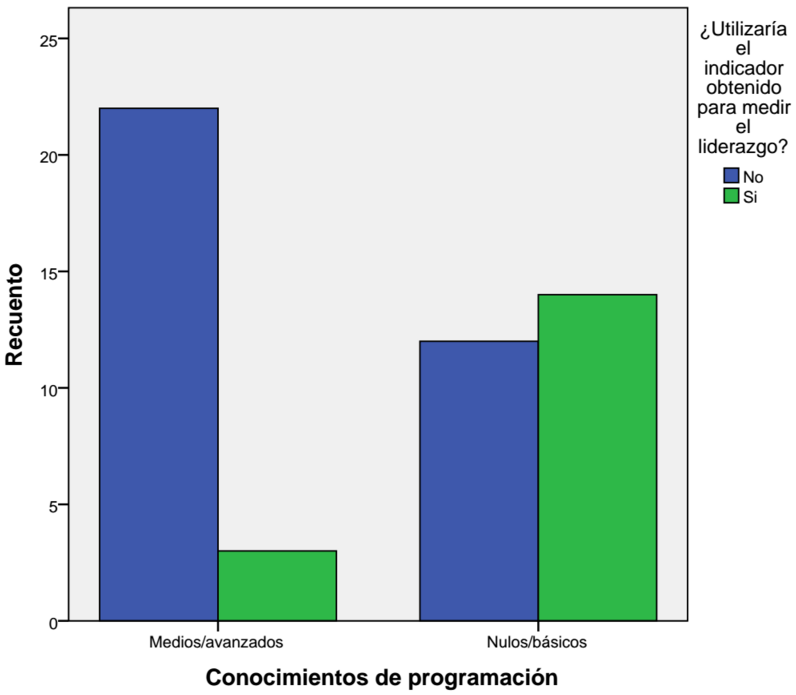
\includegraphics[scale=0.3]{barras_programacion_liderazgo.png}
  \end{center}
  \caption{Utilizaría el indicador para evaluar el liderazgo}
  \label{fig:app:barras:programacion:liderazgo}
\end{figure}

Para demostrar la independencia entre los conocimientos de programación y la validez que da el participante al indicador para evaluar dicha competencia vamos a definir la siguiente hipótesis nula:

\begin{mdframed}[style=hipotesis0]
$H_0$: \emph{Los \textbf{conocimientos de programación} son independientes de que el individuo considere que les son válidos los indicadores extraídos para medir la competencia de \textbf{liderazgo}}
\end{mdframed}

Para contrastar la hipótesis nula se utilizará la prueba de chi-cuadrado. Se construye la tabla de contingencia y se calculan las frecuencias esperadas, obteniéndose el siguiente valor de chi-cuadrado ($\chi^2_0$): 

\begin{center}
	\framebox[1.2\width]{$\chi^2_0 = 10,043$}
\end{center}

Para contrastar la hipótesis se utiliza un nivel de significación del 5\percentage, siendo este valor 3,84. 

\begin{center}
	\framebox[1.2\width]{$\chi^2_{\alpha (r-1)(c-1)} = \chi^2_{0,05 (2-1)(2-1)} = 3,84$}
\end{center}

Como 10,043 es mayor que 3,84 se rechaza la hipótesis nula, y se concluye que con una significación del 5\percentage no se puede asegurar que los datos sean independientes.

\begin{center}
	\framebox[1.2\width]{$\chi^2_0 > \chi^2_{0,05 (2-1)(2-1)} \Rightarrow  10,043 > 3,84$}
\end{center}

Para no rechazar la hipótesis nula debería tomarse un nivel de significación del 0,1\percentage, siendo este valor 10,827.

\begin{center}
	\framebox[1.2\width]{$\chi^2_0 \leq \chi^2_{0,001 (2-1)(2-1)} \Rightarrow  10,043 \leq 10,827$}
\end{center}

% -----  ----------
% ----- PERFIL ----------
% ----- ----------

\subsubsection{Perfil}

\paragraph*{Trabajo en equipo}

En la figura~\ref{fig:app:barras:perfil:equipo} se pueden ver las respuestas de los participantes a si utilizarían o no el indicador proporcionado para evaluar el trabajo en equipo de los usuarios del wiki en base a su perfil.

\begin{figure}
  \begin{center}
    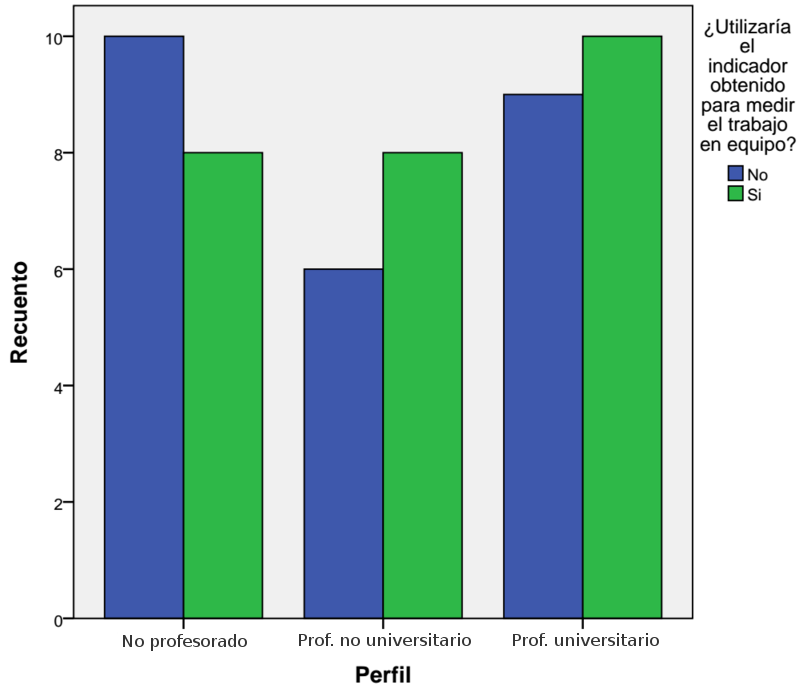
\includegraphics[scale=0.3]{barras_perfil_equipo.png}
  \end{center}
  \caption{Utilizaría el indicador para evaluar el trabajo en equipo}
  \label{fig:app:barras:perfil:equipo}
\end{figure}

Para demostrar la independencia entre el perfil y la validez que da el participantes al indicador para evaluar dicha competencia vamos a definir la siguiente hipótesis nula:

\begin{mdframed}[style=hipotesis0]
$H_0$: \emph{El \textbf{perfil} del individuo es independiente de que el individuo considere que les son válidos los indicadores extraídos para medir la competencia de \textbf{trabajo en equipo}}
\end{mdframed}

Para contrastar la hipótesis nula se utilizará la prueba de chi-cuadrado. Se construye la tabla de contingencia y se calculan las frecuencias esperadas, obteniéndose el siguiente valor de chi-cuadrado ($\chi^2_0$): 

\begin{center}
	\framebox[1.2\width]{$\chi^2_0 = 0,541$}
\end{center}

Para contrastar la hipótesis se utiliza un nivel de significación del 5\percentage, siendo este valor 5,991. 

\begin{center}
	\framebox[1.2\width]{$\chi^2_{\alpha (r-1)(c-1)} = \chi^2_{0,05 (2-1)(3-1)} = 5,991$}
\end{center}

Como 0,541 es menor que 5,991 no se rechaza la hipótesis nula, y se concluye que con una significación del 5\percentage los datos son independientes.

\begin{center}
	\framebox[1.2\width]{$\chi^2_0 \leq \chi^2_{0,05 (2-1)(3-1)} \Rightarrow  0,541 \leq 5,991$}
\end{center}
 
\paragraph*{Planificación y gestión del tiempo}
 
En la figura~\ref{fig:app:barras:perfil:planificacion} se pueden ver las respuestas de los participantes a si utilizarían o no el indicador proporcionado para evaluar la planificación y gestión del tiempo de los usuarios del wiki en base a su perfil.

\begin{figure}
  \begin{center}
    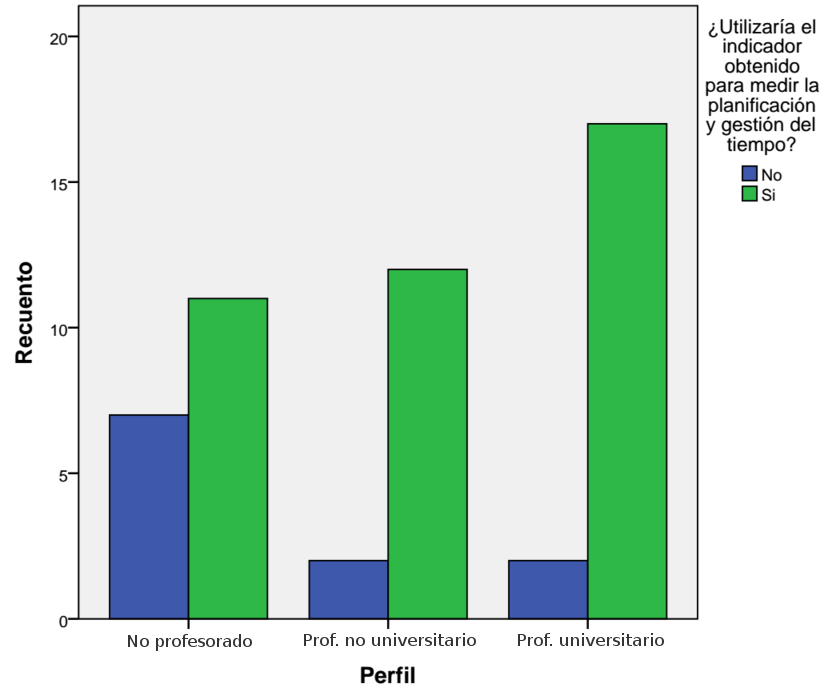
\includegraphics[scale=0.3]{barras_perfil_planificacion.png}
  \end{center}
  \caption{Utilizaría el indicador para evaluar la planificación y gestión de tiempo}
  \label{fig:app:barras:perfil:planificacion}
\end{figure}

Para demostrar la independencia entre los conocimientos de programación y la validez que da el participante al indicador para evaluar dicha competencia vamos a definir la siguiente hipótesis nula:

\begin{mdframed}[style=hipotesis0]
$H_0$: \emph{El \textbf{perfil} del individuo es independiente de que el individuo considere que les son válidos los indicadores extraídos para medir la competencia de \textbf{planificación y gestión del tiempo}}
\end{mdframed}

Para contrastar la hipótesis nula se utilizará la prueba de chi-cuadrado. Se construye la tabla de contingencia y se calculan las frecuencias esperadas, obteniéndose el siguiente valor de chi-cuadrado ($\chi^2_0$): 

\begin{center}
	\framebox[1.2\width]{$\chi^2_0 = 5,001$}
\end{center}

Para contrastar la hipótesis se utiliza un nivel de significación del 5\percentage, siendo este valor 5,991. 

\begin{center}
	\framebox[1.2\width]{$\chi^2_{\alpha (r-1)(c-1)} = \chi^2_{0,05 (2-1)(3-1)} = 5,991$}
\end{center}

Como 5,001 es menor que 5,991 no se rechaza la hipótesis nula, y se concluye que con una significación del 5\percentage  los datos son independientes.

\begin{center}
	\framebox[1.2\width]{$\chi^2_0 \leq \chi^2_{0,05 (2-1)(2-1)} \Rightarrow  5,001 \leq 5,991$}
\end{center}

\paragraph*{Liderazgo}
 
En la figura~\ref{fig:app:barras:perfil:liderazgo} se pueden ver las respuestas de los participantes a si utilizarían o no el indicador proporcionado para evaluar el liderazgo de los usuarios del wiki en base a su perfil.

\begin{figure}
  \begin{center}
    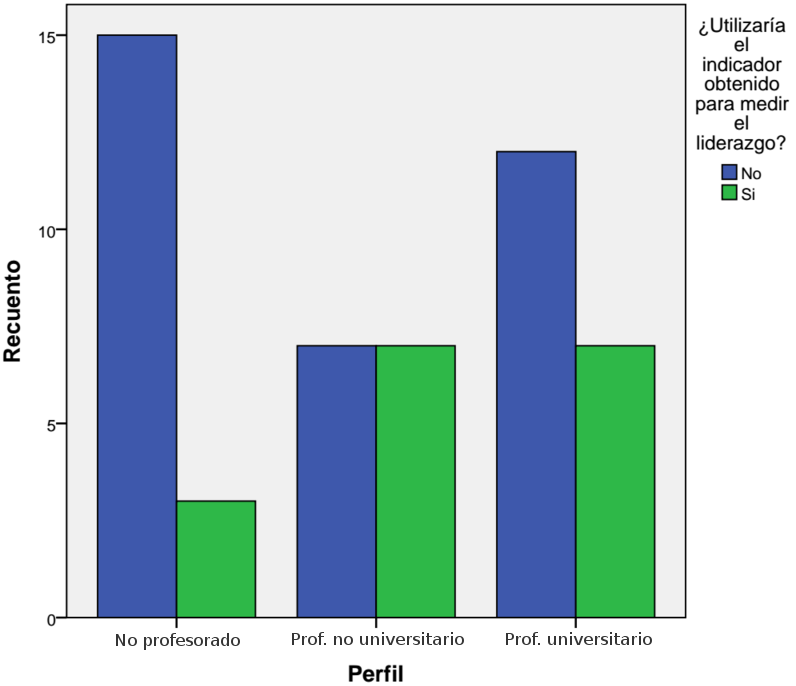
\includegraphics[scale=0.3]{barras_perfil_liderazgo.png}
  \end{center}
  \caption{Utilizaría el indicador para evaluar el liderazgo}
  \label{fig:app:barras:perfil:liderazgo}
\end{figure}

Para demostrar la independencia entre el perfil y la validez que da el participante al indicador para evaluar dicha competencia vamos a definir la siguiente hipótesis nula:

\begin{mdframed}[style=hipotesis0]
$H_0$: \emph{El \textbf{perfil} del individuo es independiente de que el individuo considere que les son válidos los indicadores extraídos para medir la competencia de \textbf{liderazgo}}
\end{mdframed}

Para contrastar la hipótesis nula se utilizará la prueba de chi-cuadrado. Se construye la tabla de contingencia y se calculan las frecuencias esperadas, obteniéndose el siguiente valor de chi-cuadrado ($\chi^2_0$): 

\begin{center}
	\framebox[1.2\width]{$\chi^2_0 = 4,105$}
\end{center}

Para contrastar la hipótesis se utiliza un nivel de significación del 5\percentage, siendo este valor 5,991. 

\begin{center}
	\framebox[1.2\width]{$\chi^2_{\alpha (r-1)(c-1)} = \chi^2_{0,05 (2-1)(3-1)} = 5,991$}
\end{center}

Como 4,105 es menor que 5,991 no se rechaza la hipótesis nula, y se concluye que con una significación del 5\percentage los datos son independientes.

\begin{center}
	\framebox[1.2\width]{$\chi^2_0 \leq \chi^2_{0,05 (2-1)(3-1)} \Rightarrow  4,105 \leq 5,991$}
\end{center}
 
\subsubsection{Comentarios} \label{ape:cuestionario:comentarios}

Los participantes en el cuestionario tenían la posibilidad de justificar sus respuestas. A continuación se resume para cada competencia las justificaciones dadas por estos para el sí o para el no:

\paragraph*{Trabajo en equipo}

Justificaciones para el sí:

\begin{itemize}
\item Porque las aportaciones de cada uno son muy dispares, demostrando, al menos, poca coordinación entre ellos
\item Pienso que sería posible, ya que podemos comprobar el volumen de aportación de cada uno. Si más o menos los tres han aportado lo mismo, podremos decir que más o menos han trabajado en equipo
\item Puede medirse el trabajo de cada uno por separado. Sin embargo, no sabemos si son entradas modificadas o cantidad de texto. Quizá el estudiante 3 estuvo más horas trabajando o escribió más texto. Sería interesante medir la cantidad de texto modificado
\item Si se conoce quién integra los grupos es posible (aunque tal vez no muy fiable) evaluar la correlación entre las curvas de los distintos integrantes y en consecuencia el trabajo en equipo
\item Porque se percibe el grado de participación de cada integrante
\item Vemos cuánto ha aportado cada uno y en qué momentos
\item Saber si el alumno trabajó por su cuenta o realizó un esfuerzo para debatir y buscar consenso en el contenido con sus compañeros
\item Sería posible observando la proximidad de las gráficas y los bytes que alcanzan, aun en un distinto espacio temporal. Aunque podría darse el caso de que dos aportaciones con el mismo peso en bytes no se correspondan con el tiempo y esfuerzo dedicado, dado que todas las aportaciones no tienen el mismo grado de dificultad
\item Puede dar información sobre la actividad de cada usuario con respecto al tráfico de datos que ha manejado
\item Trabajo en equipo = wiki
\item Se indican las coincidencias temporales y los volúmenes de aportación de información al producto final
\item Se registra la participación individual de cada alumno al resultado conjunto de grupo
\item A la vista de la gráfica, suponiendo que se trate de un equipo de trabajo, puede valorarse el grado de implicación, constancia y aportación de cada miembro
\item Pienso que evaluar la competencia del trabajo en equipo implica evaluar tanto el resultado como el proceso de trabajo. Esta herramienta se centra en el resultado y evidencia el momento en el que se realiza cada una de las aportaciones. Sin embargo, a partir de dichos gráficos, no podríamos  derivar aspectos ligados al proceso de trabajo como la capacidad de sus miembros para la planificación, coordinación, liderazgo, resolución de conflictos, etc.
\item Si los estudiantes verdaderamente han trabajado en equipo los gráficos anteriores deben de reflejar esa contribución colectiva, bien reflejada en tiempos distintos de trabajo más intenso, bien reflejando trabajo en los mismos tiempos, dependiendo de la naturaleza del trabajo encargado por el profesor y la naturaleza de la contribución/colaboración esperada
\item El gráfico facilita tanto información sobre el número de entradas de cada usuario como el número de aportaciones de cada uno
\item Se observa que uno de los usuarios ha realizado de manera periódica aportaciones considerables. Los otros dos han participado con menos peso  en las mismas fechas. Se puede pensar que el ejecutor principal de la wiki es el 1 y los otros dos aportan ideas 
\item El trabajo en equipo supone interacción entre los participantes. No me veo capaz de discernir con precisión el grado de interacción con la información proporcionada, ya que quizás distribuyeron previamente el trabajo a realizar, pero por la distribución de trabajo no se ve mucha interacción entre ellos
\item En los gráficos se puede observar la carga de trabajo de cada miembro del grupo
\end{itemize}

Justificaciones para el no:

\begin{itemize}
\item No se puede establecer una relación directa entre la participación individual y la interacción con otros	
\item La mera aportación individual de cada estudiante no parece indicar el trabajo en equipo, ya que pudieron haber realizado las ediciones de forma coordinada o como "lobos solitarios"
\item Porque la cantidad de información aportada o el momento en que se haya incluido no tienen que ver con esta competencia, y tampoco la coincidencia de ediciones en el tiempo (que puede ser eso, coincidencia, o bien justo lo contrario a saber trabajar en equipo, es decir, conflictos)
\item No sabemos en qué espacio de nombres se aportaron esos bytes
\item Porque no hay nada que indique interacción, sino acción
\item No se ve sobre qué páginas han interaccionado ni cómo lo han hecho
\item El volumen de aportación no es indicativo del trabajo en equipo porque no hay datos de la calidad de la información aportada. Sí es indicativo de un uso no equitativo. Y aunque la calidad aportada fuera similar, el trabajo en equipo depende del equipo de trabajo. No hay una única forma de trabajar en equipo, por lo que el gráfico no es indicativo
\item No hay datos sobre el tema
\item Es necesario conocer qué tipo de trabajo y la composición y roles en el grupo
\item Se puede observar las aportaciones individuales de cada uno pero no el trabajo colaborativo entre ellos que sería lo importante del trabajo en equipo.
\item Porque cada alumno podría haber trabajado en áreas totalmente distintas, haciendo un trabajo individual
\item De los gráficos anteriores no se puede inferir qué cantidad de trabajo han realizado los alumnos en equipo; es posible que cada uno haya realizado sus tareas individualmente por separado
\item Se puede dar la circunstancia de que los tres trabajen en equipo y sólo uno transcribe las aportaciones, por tanto en el gráfico sólo aparecería la aportación de uno de ellos
\item Porque sería las aportaciones de los alumnos de forma individualizada. Creo que podría haber otros indicadores para el trabajo en equipo. Las anotaciones entre alumnos u otro indicador parecido
\item Los gráficos recogen las aportaciones de los alumno individualmente
\item Por que conoces en qué momento entran y suben cosas, pero no si están trabajando de forma conjunta
\end{itemize}

\paragraph*{Planificación y gestión del tiempo}

Justificaciones para el sí:

\begin{itemize}
\item El usuario 1 realiza contribuciones periódicas todo lo contrario que el usuario 3
\item Porque se muestra una periodización del trabajo de cada uno
\item Estudiando la distribución a través del tiempo de las ediciones se puede uno hacer una idea bastante clara de la planificación del tiempo
\item Porque se aprecia fácilmente la distribución de las contribuciones en el tiempo
\item Podemos ver si se han planificado para trabajar durante el período estipulado de forma continua o si han tenido picos de trabajo puntuales justo antes de entregar
\item Puede verse si se ha hecho todo al final o al principio de la temporización
\item La herramienta permite identificar si el estudiante trabajó por picos o de manera continua, de lo que puede inferirse una planificación (o ausencia de ella) anterior
\item Porque es posible observar las variaciones en la actividad
\item Vemos cuánto ha aportado cada uno y en qué momentos
\item Sería posible observando la línea temporal de aportaciones al wiki, comprobando si la carga de trabajo se ha distribuido de forma homogénea a lo largo del tiempo
\item El gráfico refleja la planificación y gestión del tiempo de cada alumno
\item Se indican cronológicamente los accesos al objeto del trabajo y los volúmenes aportados
\item Con las gráficas podemos observar en cada semana el trabajo que ha aportado cada estudiante y se observa el estudiante que ha tenido un trabajo continuado al igual que el que ha realizado su máxima aportación en un periodo concreto
\item A lo largo del eje temporal se puede valorar la administración del tiempo de trabajo de cada alumno
\item Puede valorarse si el trabajo ha sido periódico o si se trata de un trabajo hecho en un momento o día determinado
\item Porque podemos ver cuándo le han dedicado tiempo al trabajo. No se ven las horas, pero podríamos estimarlas a partir del contenido añadido
\item Por el mismo motivo que en el caso anterior. Muestra cómo el estudiante ha empleado el tiempo en su wiki, y se puede valorar si es así o no como debía haberlo hecho
\item El gráfico parece indicar que mientras el usuario 1 realiza su actividad en el wiki de forma constante y durante un tiempo más extendido, no ocurre lo mismo con los usuarios 1 y 2, que empiezan a trabajar mucho más tarde y con menos intensidad
\item Según las gráficas si se observa una simultaneidad en las aportaciones. Por lo que se puede suponer que entre ellos existió una coordinación y planificación del trabajo
\item En efecto, los gráficos muestran la cantidad de tiempo que los alumnos invierten en sus tareas a lo largo de un período determinado; a partir de aquí podríamos evaluar su capacidad de planificación y gestión del tiempo.
\item Bueno el 1 ha ido haciendo aportaciones regulares y el 3 sólo al final. Pero puede ser que el reparto que se hicieron del trabajo era precisamente que el 1 buscara la información y el 3 desarrollara conclusiones. Pero bueno, entonces tendría que haber actuado al final y no en el punto intermedio
\item Se observa claramente la distribución en el tiempo del trabajo realizado
\item Es fácil comprobarlo viendo la frecuencia de aportaciones, momento, etc
\item Podríamos comprobar que cada alumno ha estado desarrollando actividades de Wiki a lo largo del tiempo y en qué momento ha trabajado en la actividad
\item Los gráficos muestran los bytes que cargan los alumnos por semana
\item Sabemos en qué momento entran, por tanto, si concentran el trabajo o lo hacen de forma continua a lo largo del tiempo establecido.
\end{itemize}

Justificaciones para el no:

\begin{itemize}
\item Los gráficos no muestran la gestión del tiempo, es decir, el tiempo dedicado por cada estudiante. La competencia de planificación me resulta un término difícil de entender
\item Puedo invertir mucho tiempo en programar al principio y luego es simplemente correr el robot
\item Se puede verificar en el caso de mayor participación, pero no hay elementos suficientes en los otros casos
\item Ni sí ni no... Habrá que ver cómo está organizado el curso y la planificación de actividades
\item Los gráficos indican un resultado a posteriori de la participación. Ésta puede haberse visto influida por múltiples factores (otros trabajos o entregas, circunstancias personales, etc.). No ofrece ninguna información fiable sobre el grado de planificación y gestión del tiempo del alumno
\item Imposible si no se conoce la planificación previa de cada estudiante
\item Sin saber en qué consiste el trabajo no se podría saber. Entiendo que no debería haber una única planificación/gestión que actúe como molde evaluador
\item Al igual que dije anteriormente, por poner el foco en el resultado y no en el proceso. No puedo saber si ha habido una planificación (previa o durante la construcción del wiki). Sería interesante conocer el acuerdo al que ha llegado el equipo (o los acuerdos que se van tomando sobre la marcha) de cara a planificar su trabajo y gestión del tiempo, comprobando si efectivamente el resultado se ajusta a lo planificado
\end{itemize}

\paragraph*{Liderazgo}

Justificaciones para el sí:

\begin{itemize}
\item Porque un estudiante destaca por encima de los otros dos, pudiendo deberse a un rol de liderazgo
\item Puede distinguirse quien ha trabajado más (normalmente el líder, siempre y cuando se mida realmente la cantidad de trabajo en los gráficos, como he dicho anteriormente)
\item Entiendo que sí sería posible, ya que el recorrido de cada gráfica nos indicaría si alguno de los participantes suele adelantarse a sus compañeros en las aportaciones, lo que podría significar un liderazgo en el proyecto.
\item Mediante el nivel de participación en el propio tráfico de datos ...
\item De acuerdo a la mayor o menor participación y trabajo = liderazgo
\item Por la mayor participación 
\item Puede observarse quién se ha implicado más en el proyecto y quiénes no lo han hecho
\item Supongo que el que lleva el papel de líder reflejará un mayor tiempo de dedicación, tiempo que emplearía en revisar y comprobar las contribuciones de sus compañeros
\item Al parecer los usuarios 2 y 3 aumentan su actividad conforme que vaya aumentando su actividad el usuario 1, que parece ser el más activo.
\item Generalmente el alumno que adopta el papel de líder asume más responsabilidad y, por tanto, acaba aportando más en los trabajos por equipo.
\item Lo que se ve es que el usuario 1 ha cargado casi todo el trabajo, pero insisto en que depende de qué trabajo es el que ha hecho. Puede haber sido buscar información y subirla, y el 3 analizarla que supone en definitiva más trabajo intelectual. Pero si hubiera tenido capacidad de liderazgo el trabajo hubiera sido más fluido
\item Entiendo que sí. Supongo que sería aquel que más aportaciones haga de forma más continuada
\item Se podría comprobar a partir del cual  quien ha participado con mayores contribuciones y más valiosas, así como el seguimiento de sus ideas a través de las relaciones establecidas
\end{itemize}

Justificaciones para el no:

\begin{itemize}
\item No se puede establecer una relación directa entre la participación individual y la interacción con otros
\item No veo forma de evaluar factores como el liderazgo a partir del número de ediciones, sin factores más cualitativos
\item Los gráficos muestra qué estudiante ha sido el más activo, es decir el más trabajador. Ahora bien, de ahí deducir su liderazgo, no es plausible
\item Porque esta competencia no se refleja en los bytes aportados ni en su distribución en el tiempo, no puede conocerse quién promueve qué. Incluso los usuarios que menos información han aportado podrían haber centrado sus esfuerzos en ayudar a todos los demás, así como los que más información han aportado podrían haber actuado también como líderes predicando con el ejemplo
\item Puedo invertir mucho tiempo en programar al principio y luego es simplemente correr el robot
\item El liderazgo se puede ejercer de muchas maneras, pero rara vez viene dado por el peso directo del trabajo propio, que es de lo que dan idea los gráficos
\item No creo que sería posible medir el liderazgo en esos gráficos, ya que no sabemos las motivaciones para participar en el trabajo (si los ha animado cualquier compañero y cuál de ellos)
\item No veo cómo podría evaluarse dicha competencia a la vista de las gráficas, a menos que identifiquemos cantidad de participaciones con características de liderazgo, lo cual me parece un tanto arriesgado
\item Porque no hay forma de saber quién dirige los trabajos. Aunque se podría inferir dada la mayor intervención de algún integrante, las razones para una mayor intervención pueden ser justo por una falta de liderazgo
\item Nada me da datos al respecto
\item Se muestra simplemente quién ha aportado más (cuantitativamente) y de forma más sostenida en el tiempo, pero no aporta información relativa a quién ha dirigido la discusión o ha mostrado más capacidad de liderazgo. Solo mide actividad y numero de aportaciones, que puede ser parte de la evaluación de liderazgo pero no la define por completo
\item No hay datos
\item Porque no sabemos cómo ha sido el trabajo en equipo. Se necesita de observación
\item El liderazgo no implica que un miembro del equipo haga más cosas visibles, podría ser lo contrario
\item Necesitaría información sobre las interacciones entre los estudiantes
\item Creo que esta competencia se observaría de forma directa en el trabajo en equipo. Sería la forma de ver quién ejerce el rol de líder, de organizar el trabajo, mediar ante las distintas opiniones y facilitar que el grupo llegue a un acuerdo.
\item Porque no conocemos siquiera si ha existido comunicación entre ellos
\item Incidiendo nuevamente en las anteriores ideas plasmadas. ¿Cómo podría, por ejemplo, saber si un determinado miembro del equipo tiene capacidad para motivar a los demás para la consecución del objetivo común?. ¿Cómo podría saber quién toma las decisiones más importantes?. ¿Podríamos saber quién deja de ser un líder y cuándo otro asume dicho rol?
\item A simple vista se aprecia quien ha hecho más aportaciones pero no quiere decir que haya sido el que ha liderado el trabajo. Valorar por suposiciones puede llevar a equívocos
\item Creo que es difícil obtener información sobre quién ha liderado el grupo
\item Los gráficos muestran el trabajo individual de los alumnos
\item No es posible conocer las relaciones que se establecen entre ellos
\end{itemize}